
%%% Chapter 2: Towards Human-AI Teaming for Cybersecurity
%%% Based on: "Towards Human-AI Teaming for Cybersecurity" (DESTION 2026)
%%% Authors: Himanshu Neema, Akhilesh Raj (Vanderbilt University)

\chapter{Towards Human-AI Teaming for Cybersecurity} \label{CH2_HumanAI}

% Set the figure path for this chapter
\graphicspath{{Papers/HumanAI/}}

\section*{Abstract}
Advances in autonomous cyber defense have enabled intelligent “Blue agents” capable of monitoring large-scale networks, detecting anomalies, and rapidly deploying defensive actions. However, operational realities in enterprise, operational technology (OT), and green-field environments demonstrate that fully autonomous cyber defense remains insufficient due to contextual ambiguity, adversarial manipulation risks, and the need for strategic judgment. This paper presents a comprehensive framework for Human-AI Teaming for cyber defense, integrating a Blue agent with live network observations, risk analytics, and interactive human decision support. A unified dashboard provides multi-resolution cyber situational awareness, including node compromise states, attack traces, and dynamically scored defensive action options. Humans intervene when risk metrics, network health indicators, or mission priorities deem autonomous actions insufficient or unsafe. The platform incorporates risk-management methods as well as human-agent interaction datasets to support trust calibration and learning cycles. We demonstrate these Human-AI teaming capabilities of our platform through a case study, where we also show when and how a human can override agent's actions. The paper illustrates that well-designed Human-AI coordination can reduce cognitive load on defenders, improve resilience to adversarial attacks, and balance autonomous speed with human's contextual domain knowledge.

\section{Introduction}
Modern cyber defense operations face an unprecedented scale, velocity, and complexity of threats across enterprise networks, operational technology (OT) infrastructures, and emerging green-field digital environments. 
Despite mature monitoring tools and extensive visibility into network topology, device states, and workflow dependencies, the growing sophistication of cyber adversaries requires a defense strategy that is both proactive and adaptive.
Autonomous cyber-defense agents (referred to here as Blue agents) have emerged as a promising capability, offering continuous monitoring, rapid mitigation, and the ability to detect subtle anomalies unnoticed by humans.

Yet, autonomous agents alone cannot ensure resilient defense. 
They can suffer from false positives and false negatives, remain vulnerable to adversarial machine-learning attacks, and often lack the overall mission context or understanding of broader operational constraints. 
Defensive actions taken without contextual awareness (such as isolating key OT assets or resetting mission-critical processes) may cause more harm than the attack itself.
Meanwhile, human cyber operators (with rich contextual understanding, creativity, and ethical judgment) are still constrained by cognitive limits, fatigue, and response speed. Thus, a systematic approach to Human-AI teaming can overcome these limitations faced by humans and AI agents alone.

The core idea of Human-AI teaming is to leverage complementary strengths.
AI agents provide highly scalable and automated cybersecurity, 24/7 vigilance, and sophisticated anomaly detection. Humans provide the application context, multi-domain reasoning, and strategic decision-making. 
The teaming objective is not merely human oversight of AI, but a synergistic workflow where humans and agents continuously support, supervise, and enhance each other. 
Roles become dynamically adjustable: humans may be \textit{in-the-loop} for high-risk events, \textit{on-the-loop} for autonomous operations requiring oversight, or \textit{out-of-the-loop} for routine low-impact anomalies.

To operationalize this paradigm, we build upon existing infrastructure developed in RAMPART \cite{neema2024rampart} including: live network observations, monitoring tools, simulation and emulation environments, asynchronous agent execution, risk-scoring methodologies, and model-based network provisioning systems.
The proposed system is a unified dashboard offering deep insights through multiple explainable methods into node states, attack trajectories, and available defensive actions.
Additionally, each agent action is annotated with the action-specific explanations (generated
using shapley values \cite{b3} and counterfactual explanations \cite{b4}) and
%by the system using a probabilistic decision-tree reward scoring \cite{bastani2018verifiable}, and
an impact on overall cybersecurity risk profile of the network \cite{neema2021model}.

This allows human operators to choose to interject when risk crosses critical thresholds, when mission priorities require human judgment, or when the agent’s recommended actions present unacceptable operational tradeoffs. 
System-level datasets of these interactions are logged for training next-generation agents, calibrating trust, and enabling transparent explainability workflows.

In this paper, we present a comprehensive Human-AI teaming platform for cybersecurity. Section II reviews the related work in Human-AI teaming and explainable AI. Section III presents the teaming architecture and methods developed in this research work including: the overall system architecture, approach to generate explanations for agent actions, design of an LLM-powered interaction tool, and an intuitive dashboard for human interaction with the agent. A case study is given in Section IV to illustrate the Human-AI teaming and when and human can override the agent's action is also presented. Finally, Section V concludes and provides directions for future work. Overall, this research work provides novel implementation methods and approaches for designing a comprehensive Human-AI teaming system for cyber defense based on explainable methods.

\section{Related Work}
The integration of agentic AI-systems capable of autonomous reasoning, planning, and action represents a transformative shift in cybersecurity operations ~\cite{lazer2026surveyagenticaicybersecurity}. 
However, the dual-use nature of these technologies necessitates structured engineering frameworks to ensure effective human-agent teaming. 
Evertsz and Thangarajah propose a BDI-based methodology that uses diagrammatic representations to present contextualized team cognition to humans, facilitating their role as peers rather than mere supervisors of artificial agents \cite{evertsz2020framework}. 
A primary barrier to successful teaming is the "black-box" nature of deep learning models, which often leads to alert fatigue and a lack of trust among security analysts. 
Recent research emphasizes Explainable AI (XAI) \cite{kalimuthu2025explainable} as the critical bridge to resolving this opacity. 
For example, studies utilizing SHAP and LIME demonstrate that providing feature-level justifications for IDS alerts can significantly improve forensic analysis and decision-making \cite{kalimuthu2025explainable}. 
Furthermore, evidence from user studies indicates that hybrid UI strategies combining confidence visualizations with structured rationales are most effective at calibrating user trust and improving decision accuracy. 
Ultimately, reliability in autonomous cybersecurity is increasingly defined as a socio-technical property. 
Adebayo’s HITL-XAI framework \cite{adebayo2026human} embeds human expertise at strategic junctures of the cyber kill chain, using XAI-driven uncertainty quantification to trigger human intervention only when the AI reaches its limits.
This collaborative paradigm is echoed in governmental principles for Operational Technology (OT), which stress that humans must remain responsible for functional safety through continuous oversight and fail-safe mechanisms. 
Together, these papers advocate for a shift from passive reporting to symbiotic collaboration, where AI amplifies human capacity while human experts provide the essential context for high-stakes reasoning.

\section{Teaming Architecture \& Methods}
The concept of Human-AI Teaming for cybersecurity is motivated by limitations on both sides of the human–machine spectrum. Cyber agents excel in high-frequency detection, large-scale log processing, and consistent execution of defensive playbooks, making them invaluable during rapidly unfolding attacks such as lateral movement, credential escalation, or large-scale scanning. However, these agents lack contextual awareness, cannot interpret multi-domain implications (e.g., mission importance of an OT asset), and may recommend actions that inadvertently disrupt operations.
In contrast, human defenders possess strong contextual understanding, creativity, intuition, and ethical judgment, especially important during complex or novel attacks. Yet they struggle with the speed and volume of modern cyber engagements and can become overloaded or inconsistent under stress.

For example, let's say a Blue agent detects a privilege escalation on a subnet supporting admin systems and safety controllers. 
It decides to isolate the segment as there is a  92\% mitigation chance and only a 35\% risk of alerting the attacker. 
However, what the agent doesn't consider is that full isolation would raise operational risk during a maintenance cycle. 
So, with this contextual knowledge the human narrows the response to a subset of hosts and applies rapid policy updates, preserving mission continuity while mitigating the threat. 
The agent executes, monitors, and logs the action, showing that collaboration, not full autonomy, is essential.

To allow for this collaboration, we develop a system where human operators can override AI teammates and inject alternative actions whenever they disagree on attack or defense trajectories. 
To support issue detection and diagnosis, we provide two forms of explanations-direct and counterfactual-for agent actions, accessible through an LLM-based chatbot for ease of use. 
Finally, we integrate these explanations into a unified dashboard, where each action is annotated with its probability of success, expected execution time, likelihood of attacker detection, and impact on overall risk profile of the network \cite{neema2021model}.
A control loop in our developed system is shown in Figure \ref{fig:human_ai_loop}.

\begin{figure}[t]
\centering
\resizebox{\columnwidth}{!}{
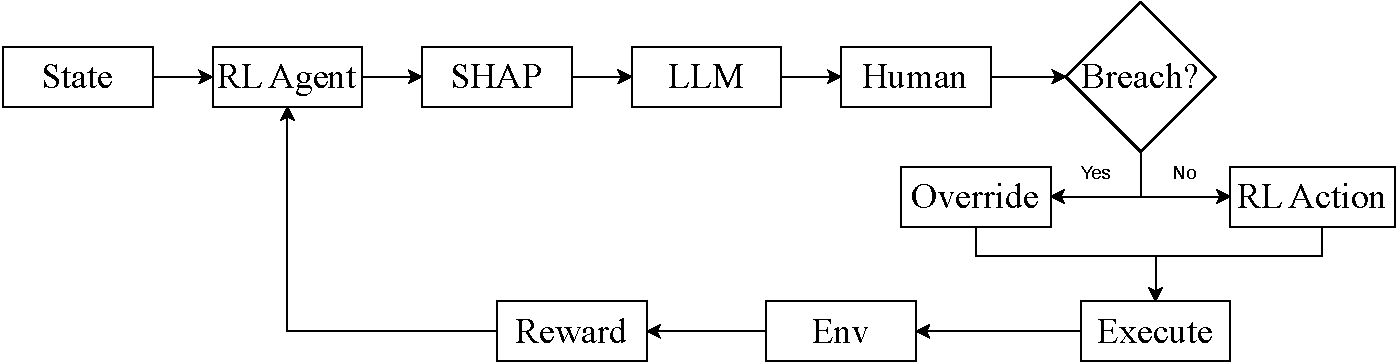
\includegraphics[]{Figures/flow_DESTION.drawio.pdf}
}
\caption{Human--AI cyber defense control loop with intervention condition.}
\label{fig:human_ai_loop}
\end{figure}

\subsection{System Architecture}
The system architecture is based on the CAGE-2 enterprise topology \cite{kiely2023autonomous} and utilizes RAMPART, a simulator to train and evaluate autonomous cyber defense agents in realistic enterprise and OT-integrated network environments.
It is deployed on an OpenStack cloud environment and consists of 15 virtual machine instances: one high-capacity Defender node and fourteen additional hosts distributed across user, enterprise, and operational subnets. 
The enterprise subnet contains mission-critical servers (enterprise0, enterprise1, enterprise2), the user subnet contains five user workstations (user0 – user4) representing typical entry points for adversarial compromise, and the operational subnet hosts OT-integrated nodes (op\_host0 - op\_host2 and op\_server0) running power grid and chemical plant control workloads. Gateway nodes interconnect these subnets, enforcing routed communication paths and enabling realistic lateral movement across network boundaries. 
A separate control network provides management-plane connectivity for orchestration, monitoring, and persistent Velociraptor communication between all endpoints and the Defender. 
The Defender node, provisioned with elevated compute resources, hosts the Velociraptor server and serves as the execution environment for the blue team actions, telemetry aggregation, logging, and reward evaluation. 
The entire topology is instantiated using OpenStack services including Nova for compute provisioning, Neutron for virtual networking and routing, and HEAT templates for declarative orchestration, enabling reproducible deployment of vulnerable services and controlled network communications. 
This emulated infrastructure preserves realistic TCP/IP routing, service discovery, exploit execution, and defensive response mechanisms, thereby providing a high-fidelity hybrid IT-OT environment for evaluating autonomous and human-in-the-loop cyber defense within RAMPART.

\subsection{Explanation Generation}
Users may request one of two types of explanations for red or blue agent actions: direct explanations (“Why does [agent] choose [action]?”) or counterfactual explanations (“Why does [agent] NOT choose [action] instead of [alternate action]?”). 
To generate these explanations, we first apply VIPER \cite{bastani2018verifiable} to distill the agent’s policy into a simple, representative decision tree. 
We then use this tree to produce either a SHAP-based direct explanation \cite{b3} or a counterfactual explanation \cite{b4}, depending on the user’s query.

RL policies are often too large and complex for human users to understand. Extracting RL policy as a decision tree can make it simple, intuitive, and easier to interpret \cite{b2}.
%Explanation generation begins by constructing a decision tree using the VIPER method that approximates the agent’s policy in a simple, interpretable form, since RL policies are often too large and complex for human users to understand \cite{b2}.
The initial tree may be empty, supplied by the user, or carried over from a previous exercise.
When the agent executes an action, we generate an abstract state that captures the context in which the action occurred. 
The features of this abstract state are binary high-level, human-readable concepts (supplied by the user or the environment) that the agent can access when selecting actions.
For example, we may track concepts such as activity, scan, and exploit detection on nodes in the network \cite{b5}. 
We determine true features in the abstract state by pattern matching against the agent's low-level observation.

We then add the abstract \{state, action\} pair to the training data for the decision tree and refit the tree using Gini impurity as the split criterion \cite{b6}.
Each internal node tests whether an abstract feature is true or false and each leaf corresponds to a possible agent action. 
Each action at a leaf is weighted by its importance, defined as the difference between its Q-value and the minimum Q-value among all available actions.
At the end of the exercise (e.g., an episode or game), we evaluate the resulting decision tree by using its representative policy (rather than the base policy) to simulate multiple attacks or defenses on the network and averaging its environmental reward.
If this new tree outperforms a tree trained on all prior data excluding the current episode, the new tree is retained as the representative policy.
Otherwise, the previous tree remains as the base. 
Repeating this update procedure after each exercise maintains an up-to-date, interpretable approximation of the underlying policy for explanation.

When the agent selects an action and the user requests a direct explanation of that selection, we apply SHAP \cite{b3} to the decision tree and return all abstract features with non-zero Shapley values. Shapley values originate from cooperative game theory and quantify the contribution of each feature to a model’s prediction by averaging its marginal impact across all possible feature subsets.
SHAP estimates each feature’s average marginal contribution on a decision by comparing the model’s prediction for the given action to a baseline prediction (the average over all actions). 
If removing a feature substantially changes the prediction, that feature receives a large-magnitude SHAP value. 
SHAP values are positive when a feature supports the chosen action and negative when it opposes it. 
Users can then inspect the features that most strongly support or oppose the action, ordered by their absolute impact.

\textit{Example 1: Consider the user query: “Why does the blue agent remove access from 'user3' when there was a scan detected on 'enterprise1'?” 
The user may be puzzled about why 'user3' is targeted instead of 'enterprise1'.
Applying SHAP to this decision yields the following normalized feature influences: scan of 'enterprise1' detected (0.655), no direct activity detected on 'enterprise0' (0.273), 'enterprise1' (0.038), 'defender' (-0.004), 'user1' (-0.007), 'user2' (-0.011), and a previous remove-action on 'user3' (-0.014).
These values indicate that the decision to remove access from 'user3' is primarily supported by the fact that a scan has occurred on 'enterprise1' but no follow-on activity has yet been observed on 'enterprise1' or 'enterprise0'. 
This suggests that the red agent may already have a foothold on 'user3' (or possibly 'user4').
The action is weakly opposed by the absence of activity elsewhere in the network and by the fact that the blue agent has already tried removing access from 'user3' once before, but not strongly enough to prevent, repeating this defensive action.}

If the user requests a counterfactual explanation \cite{b4} for a given action, we generate a set of alternative actions along with the agent’s rationale for not choosing them. 
We first enumerate all other actions with non-zero Q-values that the policy could have selected and order them by Q-value. 
For each alternative action, we use the decision tree to compute the minimal change in the abstract state required for the agent to select that action instead of the original one. 
Concretely, we identify the closest common ancestor of the two actions in the tree and report the sequence of decision nodes that must change to reach the alternative leaf. 
Users can then inspect the required feature changes and determine whether the agent should have taken an alternative action, either because its learned policy is flawed or because it lacked accurate state information when making the decision.

\textit{Example 2: Consider the user query, “Why does the blue agent remove access from 'user3' when a scan is detected on 'enterprise1'?” 
The user may believe that removing access for 'user3' is not the appropriate action and wants to understand possible alternative actions and when the agent would choose them. 
In this scenario, the agent’s policy also allows the actions of restoring 'enterprise1' and removing 'enterprise1'.
The counterfactual explanation clarifies that the agent would have restored 'enterprise1' if there had been a prior exploit on 'enterprise0'.
The agent would have removed 'enterprise1' if there were activity on 'enterprise0' or 'user3', no activity on 'user2', no prior exploits on 'enterprise0', and no scans detected on the operational server.
These explanations highlight that if the user believes, unlike the blue agent, that they know the location of the red agent, then a different action might be preferred.}

\subsection{LLM Chatbot}
Presenting users with raw numerical outputs, however, could result in significant misunderstanding.
To address this, we developed an LLM-based chatbot interface that supports natural-language question answering. 
When a user wants to know about a particular agent action, we construct a query prompt by collecting the current abstract state and the action taken by the agent. 
For counterfactual questions, we additionally extract the possible alternative actions from the agent policy.
We then instantiate one of two templates: ``Why does the agent choose [action] when in [state]?" (direct explanation) or ``Why does the agent choose [action] instead of choosing [alternate action] when in [state]?" (counterfactual explanation).
The LLM receives this prompt along with network information (e.g., machine connectivity) and the decision tree that encodes the alternative policy. 
It returns an explanation that describes why the action was taken or why an alternative was not taken in human-understandable natural language. The LLM does not generate explanations independently; instead, it translates structured outputs derived from SHAP and decision-tree policies into natural language.
In future work, for safety-critical deployment outside of the simulation environment, we plan to validate LLM outputs by ensuring consistency with the original feature set and prevent the introduction of unsupported information.

\textit{Example 3: Consider the query: ``Why does the blue agent remove access from 'user3' when there was a scan detected on 'enterprise1'?” The generated prompt is: ``Here is a decision tree showing the actions of a blue agent trying to stop a red agent on a network: [decision tree]. Here is information about the network: [network information]. Explain the following: ``Why does the agent remove 'user3' when 'enterprise1' is scanned and all other features are false?" The LLM responds: ``This could be for several reasons: (1). 'User3' might be communicating with 'Enterprise1', which could potentially be compromised by the red agent. By removing 'User3', the blue agent aims to cut off any potential communication between 'User3' and 'Enterprise1'. (2). 'User3' might be a vulnerable node in the network that could serve as an easy entry point for the red agent to move deeper into the network. By removing 'User3', the blue agent prevents this possibility. In summary, the blue agent removes 'User3' when there is no activity detected at 'Enterprise0', a scan is being performed on 'Enterprise1', and 'Enterprise1' shows some ongoing activity (indicating potential compromise or malicious action) as a precautionary measure to secure the network."}


\subsection{Dashboard}
The dashboard integrates the backend processes mentioned above using FastAPI endpoints. It is important to interact with the run-time processes in a user/operator friendly manner. The dashboard consists of an argument parser console, chatbot, a network visualizer and a status bar that aids the decision making by the operator or users.

\begin{figure*}
    \centering
    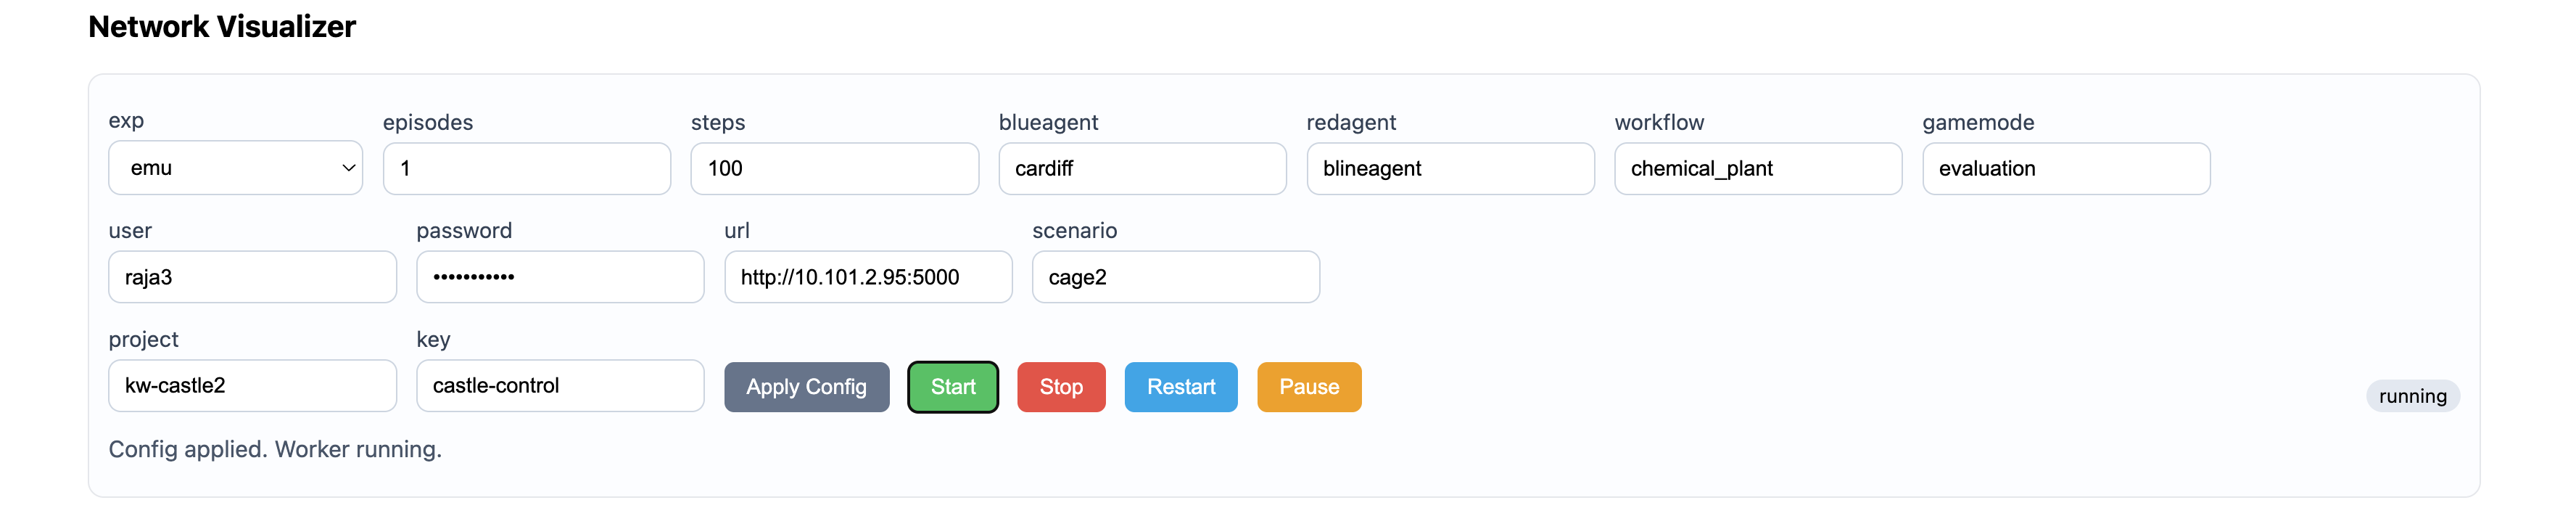
\includegraphics[width=\linewidth]{Figures/arguments.png}
    \caption{Dashboard to parse the experiment attributes.}
    \label{fig:argument_parser}
\end{figure*}

% \begin{figure*}
%     \centering
%     \includegraphics[width=\linewidth]{Figures/Network_visualizer.png}
%     \caption{Network visualizer to visualize the network topology along with red and blue attack paths.}
%     \label{fig:network_visualizer}
% \end{figure*}

% \begin{figure*}
%     \centering
%     \includegraphics[width=\linewidth]{Figures/Shap_values_actions.png}
%     \caption{Observation dashboard displaying the SHAP values and the corresponding actions.}
%     \label{fig:observation_dashboard}
% \end{figure*}

% \begin{figure*}
%     \centering
%     \includegraphics[width=\linewidth]{Figures/chat.png}
%     \caption{Chat returned by the LLM agent based on the operator query on workflow pause .}
%     \label{fig:chat_bot}
% \end{figure*}

The LLM logs (shown in Figure \ref{fig:reward_comparison}) is integrated into a browser-based operator dashboard served by a FastAPI application and accessed via a standard web interface. To enable meaningful human-in-the-loop interaction without interrupting simulation continuity, the dashboard implements a \emph{pause-and-explain} mechanism controlled by a dedicated pause toggle. When the operator activates the pause, the simulation halts at the
conclusion of the current iteration and the system enters a two-phase explanation flow. In the first phase, the dashboard immediately renders the current network state and SHAP-derived feature attributions, while displaying a visual loading indicator in place of the action selection panel; this communicates that the system is actively generating an explanation and prevents premature interaction. Concurrently, the
backend asynchronously queries the LLM with a prompt constructed from the current iteration context, including the blue and red agent actions extracted from the simulation state. In the second phase, once the LLM returns its response, the explanation text is pushed to the UI via a thread-safe snapshot bridge, the action selection panel becomes active, and the \emph{Resume} button is enabled. This sequencing ensures that operators always read the explanation before they commit to an action or continue the simulation, enforcing the intended Human-AI collaboration loop.
The synchronization between the simulation worker thread and the operator dashboard is managed through a pair of threading primitives. A \texttt{pause\_event} signals when the simulation has reached a pause point, while an \texttt{action\_selected\_event} blocks the worker until the operator has either selected an override action or clicked \emph{Resume}. A boolean flag \texttt{\_llm\_ready} gates the availability of the \emph{Resume} button in the UI, preventing the operator from advancing the simulation before the explanation has been delivered. The dashboard polls the backend at \textit{300\,ms} intervals for snapshot updates (network graph, SHAP values, available actions) and at \textit{1\,s} intervals for pause and readiness status, providing near-real-time feedback without overloading the server. Once an explanation has been displayed, it persists in the UI panel for the duration of the pause regardless of subsequent snapshot updates, so the operator can continue reading while reviewing the network visualization.

The operator action selection panel renders the set of candidate blue agent actions as clickable buttons. 
Selecting an action immediately records the operator's choice and signals the worker to resume with that action, bypassing the agent's default policy for that iteration. If no action is selected within a configurable timeout window, the simulation resumes automatically with the agent's original recommendation. 
This design preserves operational tempo while still allowing operators to intervene when the LLM explanation or SHAP attribution highlights a concern.

Together, the SHAP attributions, the decision tree policy extraction, and the LLM chatbot form a layered explanation system. SHAP values identify \emph{which features} drove the agent's decision; the decision tree renders the \emph{policy logic} in human-readable form; and the LLM chatbot translates both into \emph{natural language narrative} tailored to the operator's query. This layered approach reflects best practices in human-centered XAI, providing multiple complementary explanation modalities~\cite{ye2023complementary} while keeping the operator in meaningful control of the simulation's trajectory.
%Figure \ref{fig:argument_parser} gives quick overview of this feature.


\section{Case Study}
% To evaluate the impact of human intervention, we compare rewards from a trajectory in which all actions are selected by the agent policy with a trajectory in which a human operator can override the agent at any decision point. 
% In our evaluation scenario, the blue agent plays against a red agent using its learned policy, and we record the reward obtained when the blue agent acts autonomously. 
% Next, we have a human operator observe a replay of this game, forcing the blue agent to take the same actions as before until the first human intervention. 
% At each decision point, the operator is informed that an alternative action may be selected whenever the operator disagrees with the agent’s chosen action. 
% Whenever an override occurs, the game then evolves as if the agent had selected the human’s alternative action, and the agent resumes selecting actions autonomously until the next intervention. 
% This yields a second trajectory and an associated reward that reflects agent performance with human intervention. 
% By comparing these two rewards, we quantify the effect of human intervention on the agent’s performance. 
% The impact of human intervention is maximized when the agent’s policy is suboptimal due to factors such as limited training, noisy or inaccurate observations, or modeling errors.


To show human intervention impact, we compare rewards from a fully agent-driven trajectory with one where a human overrides action using additional contextual knowledge. This knowledge may include domain information unavailable to the RL agent, such as suspicious network traffic,
%detected by an external intrusion detection system,
historical attack patterns,
%previously observed from the red agent,
or operational priorities known to human defenders.

This study is intended as a proof-of-concept demonstration of Human-AI teaming framework rather than a statistically rigorous evaluation.
In our scenario, the blue agent plays against a red agent using its learned policy, and we record the reward obtained when the blue agent acts autonomously. The blue agent selects actions according to its reinforcement learning (RL) policy, while the red agent executes adversarial actions within the same environment. Figure~\ref{fig:environment_state} shows a representative environment state during the attack scenario.

\begin{figure}[t]
    \centering
    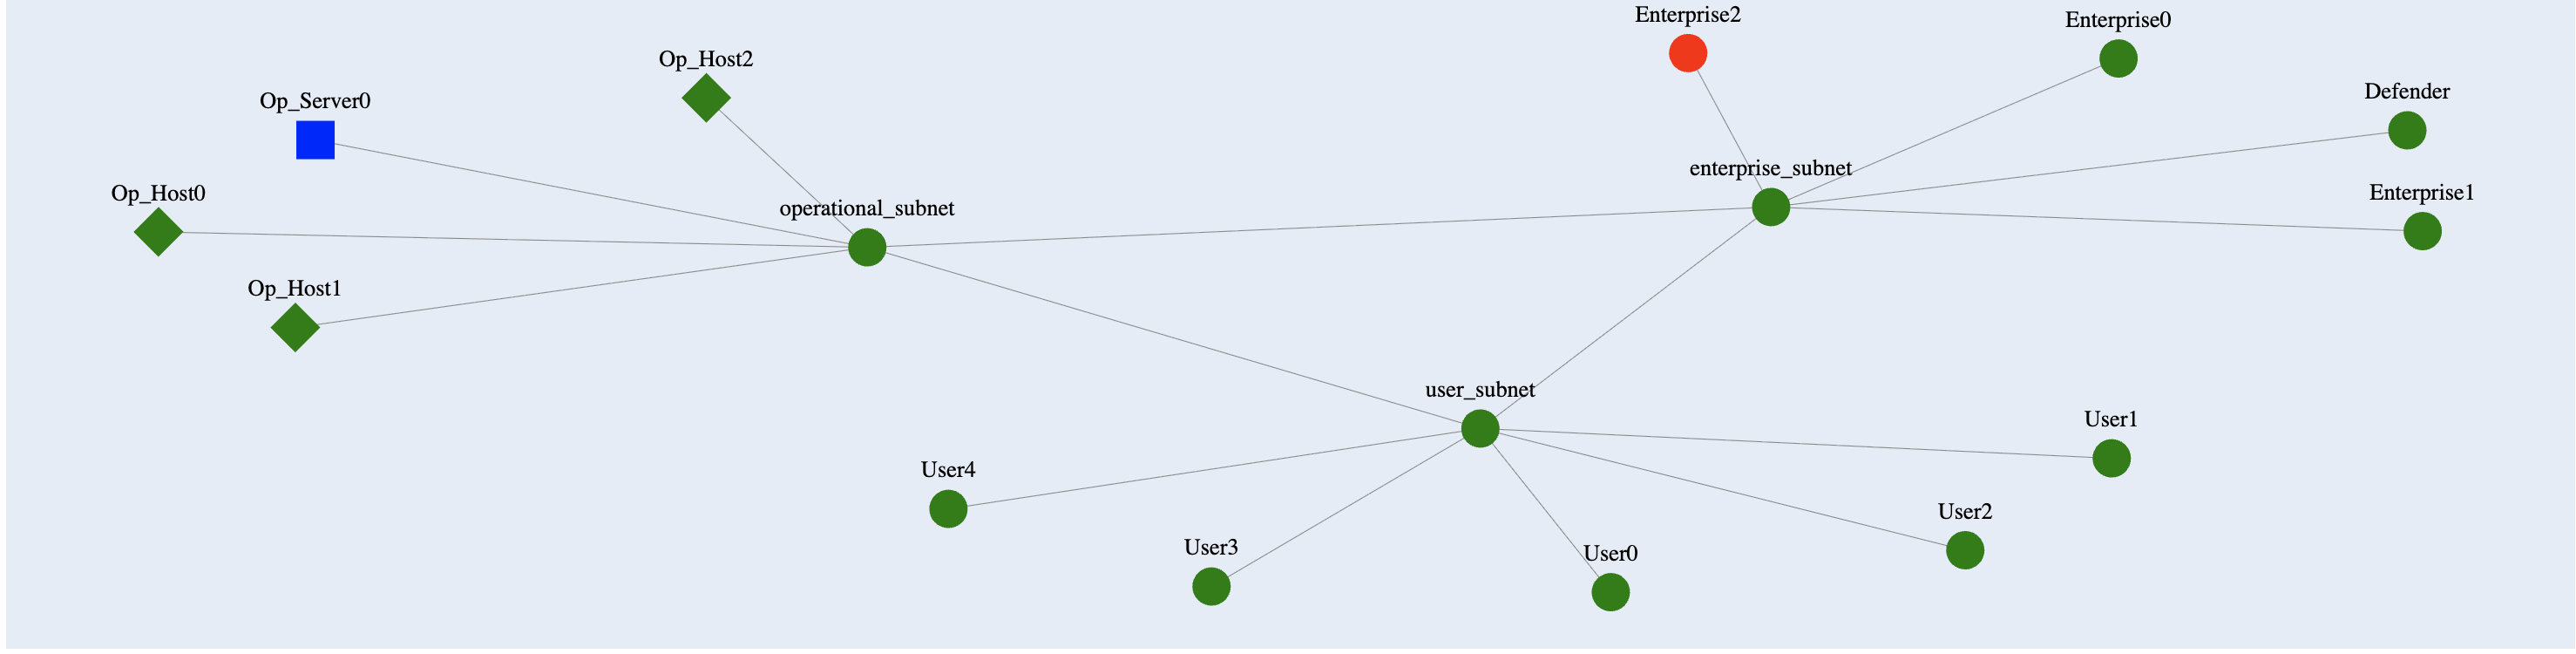
\includegraphics[width=\linewidth]{Figures/environment_state.png}
    \caption{Environment state during the attack scenario, illustrating the network topology and the red agent's activity on Enterprise2.}
    \label{fig:environment_state}
\end{figure}

Eventually, the red agent performs the action \texttt{PrivilegeEscalate\_Enterprise2} while the blue agent selects \texttt{Remove Op\_Server0}. As shown in Figure~\ref{fig:agent_action_dashboard}, this decision results in a negative step reward of $-0.1000$, indicating that the autonomous policy did not adequately mitigate the ongoing threat.

\begin{figure}[t]
    \centering
    
\includegraphics[width=\linewidth]{Figures/agent_action_dashboard.png}
    \caption{Dashboard view showing the red and blue actions at Iteration 10 and the resulting negative reward.}
    \label{fig:agent_action_dashboard}
\end{figure}

The dashboard highlights that the decision tree (DT) model disagrees with the RL agent's action and recommends an alternative such as \texttt{Ent0\_DecoyTomcat}, as illustrated in Figure~\ref{fig:dt_suggestion}. The SHAP-based explanation panel provides feature-level insight into why the RL policy chose (with an higher probability) the action \texttt{Remove Op\_Server0}, emphasizing inactivity-related features and prior user activity patterns.

\begin{figure}[t]
    \centering
    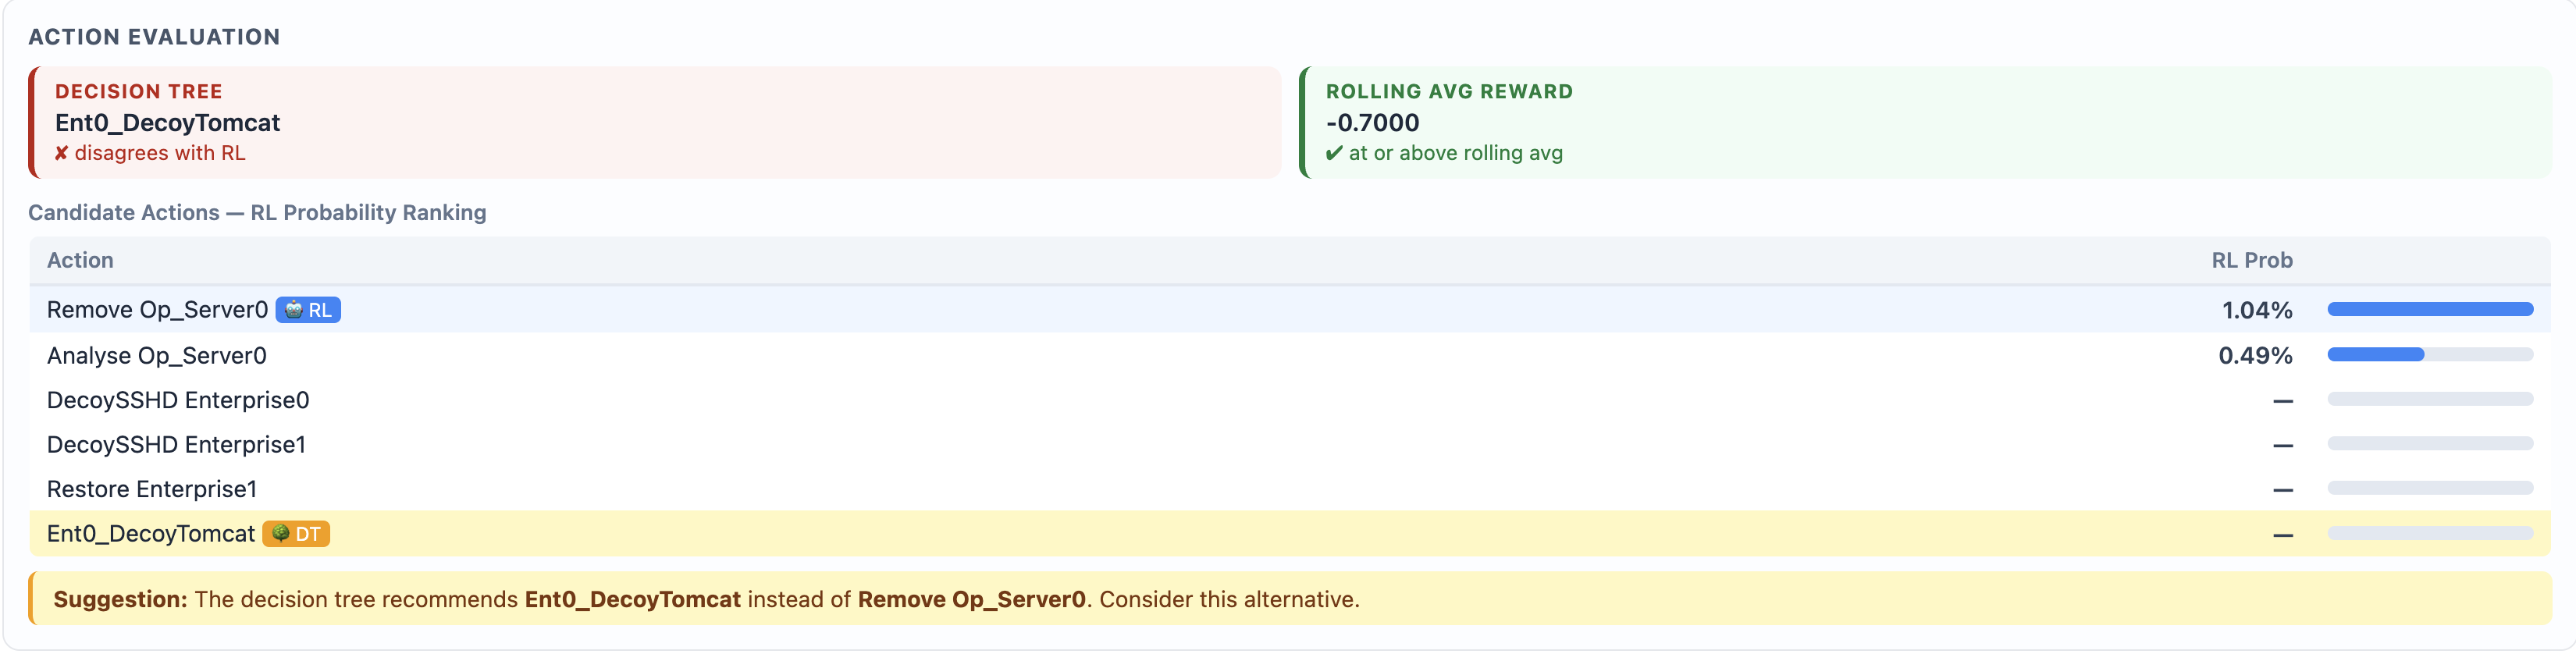
\includegraphics[width=\linewidth]{Figures/dt_suggestion.png}
    \caption{Decision tree representing the RL policy.}
    %recommendation and SHAP-based explanation highlighting feature contributions to the RL action.}
    \label{fig:dt_suggestion}
\end{figure}

However, the SHAP ranked features do not directly address the immediate adversarial activity occurring on 'Enterprise2'. The resulting negative reward demonstrates a mismatch between the learned policy's prioritization and the evolving attack context.

Next, we have a human operator observe a replay of this game, forcing the blue agent to take the same actions as before until the first human intervention. At each decision point, the operator is informed that an alternative action may be selected whenever the operator disagrees with the agent's chosen action. Figure~\ref{fig:human_override_interface} illustrates the interface that allows the operator to override the agent's action.

\begin{figure}[t]
    \centering
    
\includegraphics[width=\linewidth]{Figures/human_override_interface.png}
    \caption{Human override interface enabling intervention when the operator disagrees with the agent's selected action.}
    \label{fig:human_override_interface}
\end{figure}

When the red agent escalates privileges on 'Enterprise2', the human operator may determine, based on contextual knowledge, that the blue action should address the compromised enterprise node rather than remove an operational server.
Whenever an override occurs, the game proceeds as if the agent selected the human's alternative action, and the agent resumes selecting actions autonomously until the next intervention. This process yields a second trajectory and a reward that reflects agent performance with human intervention.

Finally, Figure~\ref{fig:dt_suggestion} conceptually illustrates the expected rewards that the human-assisted trajectory could have returned.

\begin{figure}[h]
    \centering
    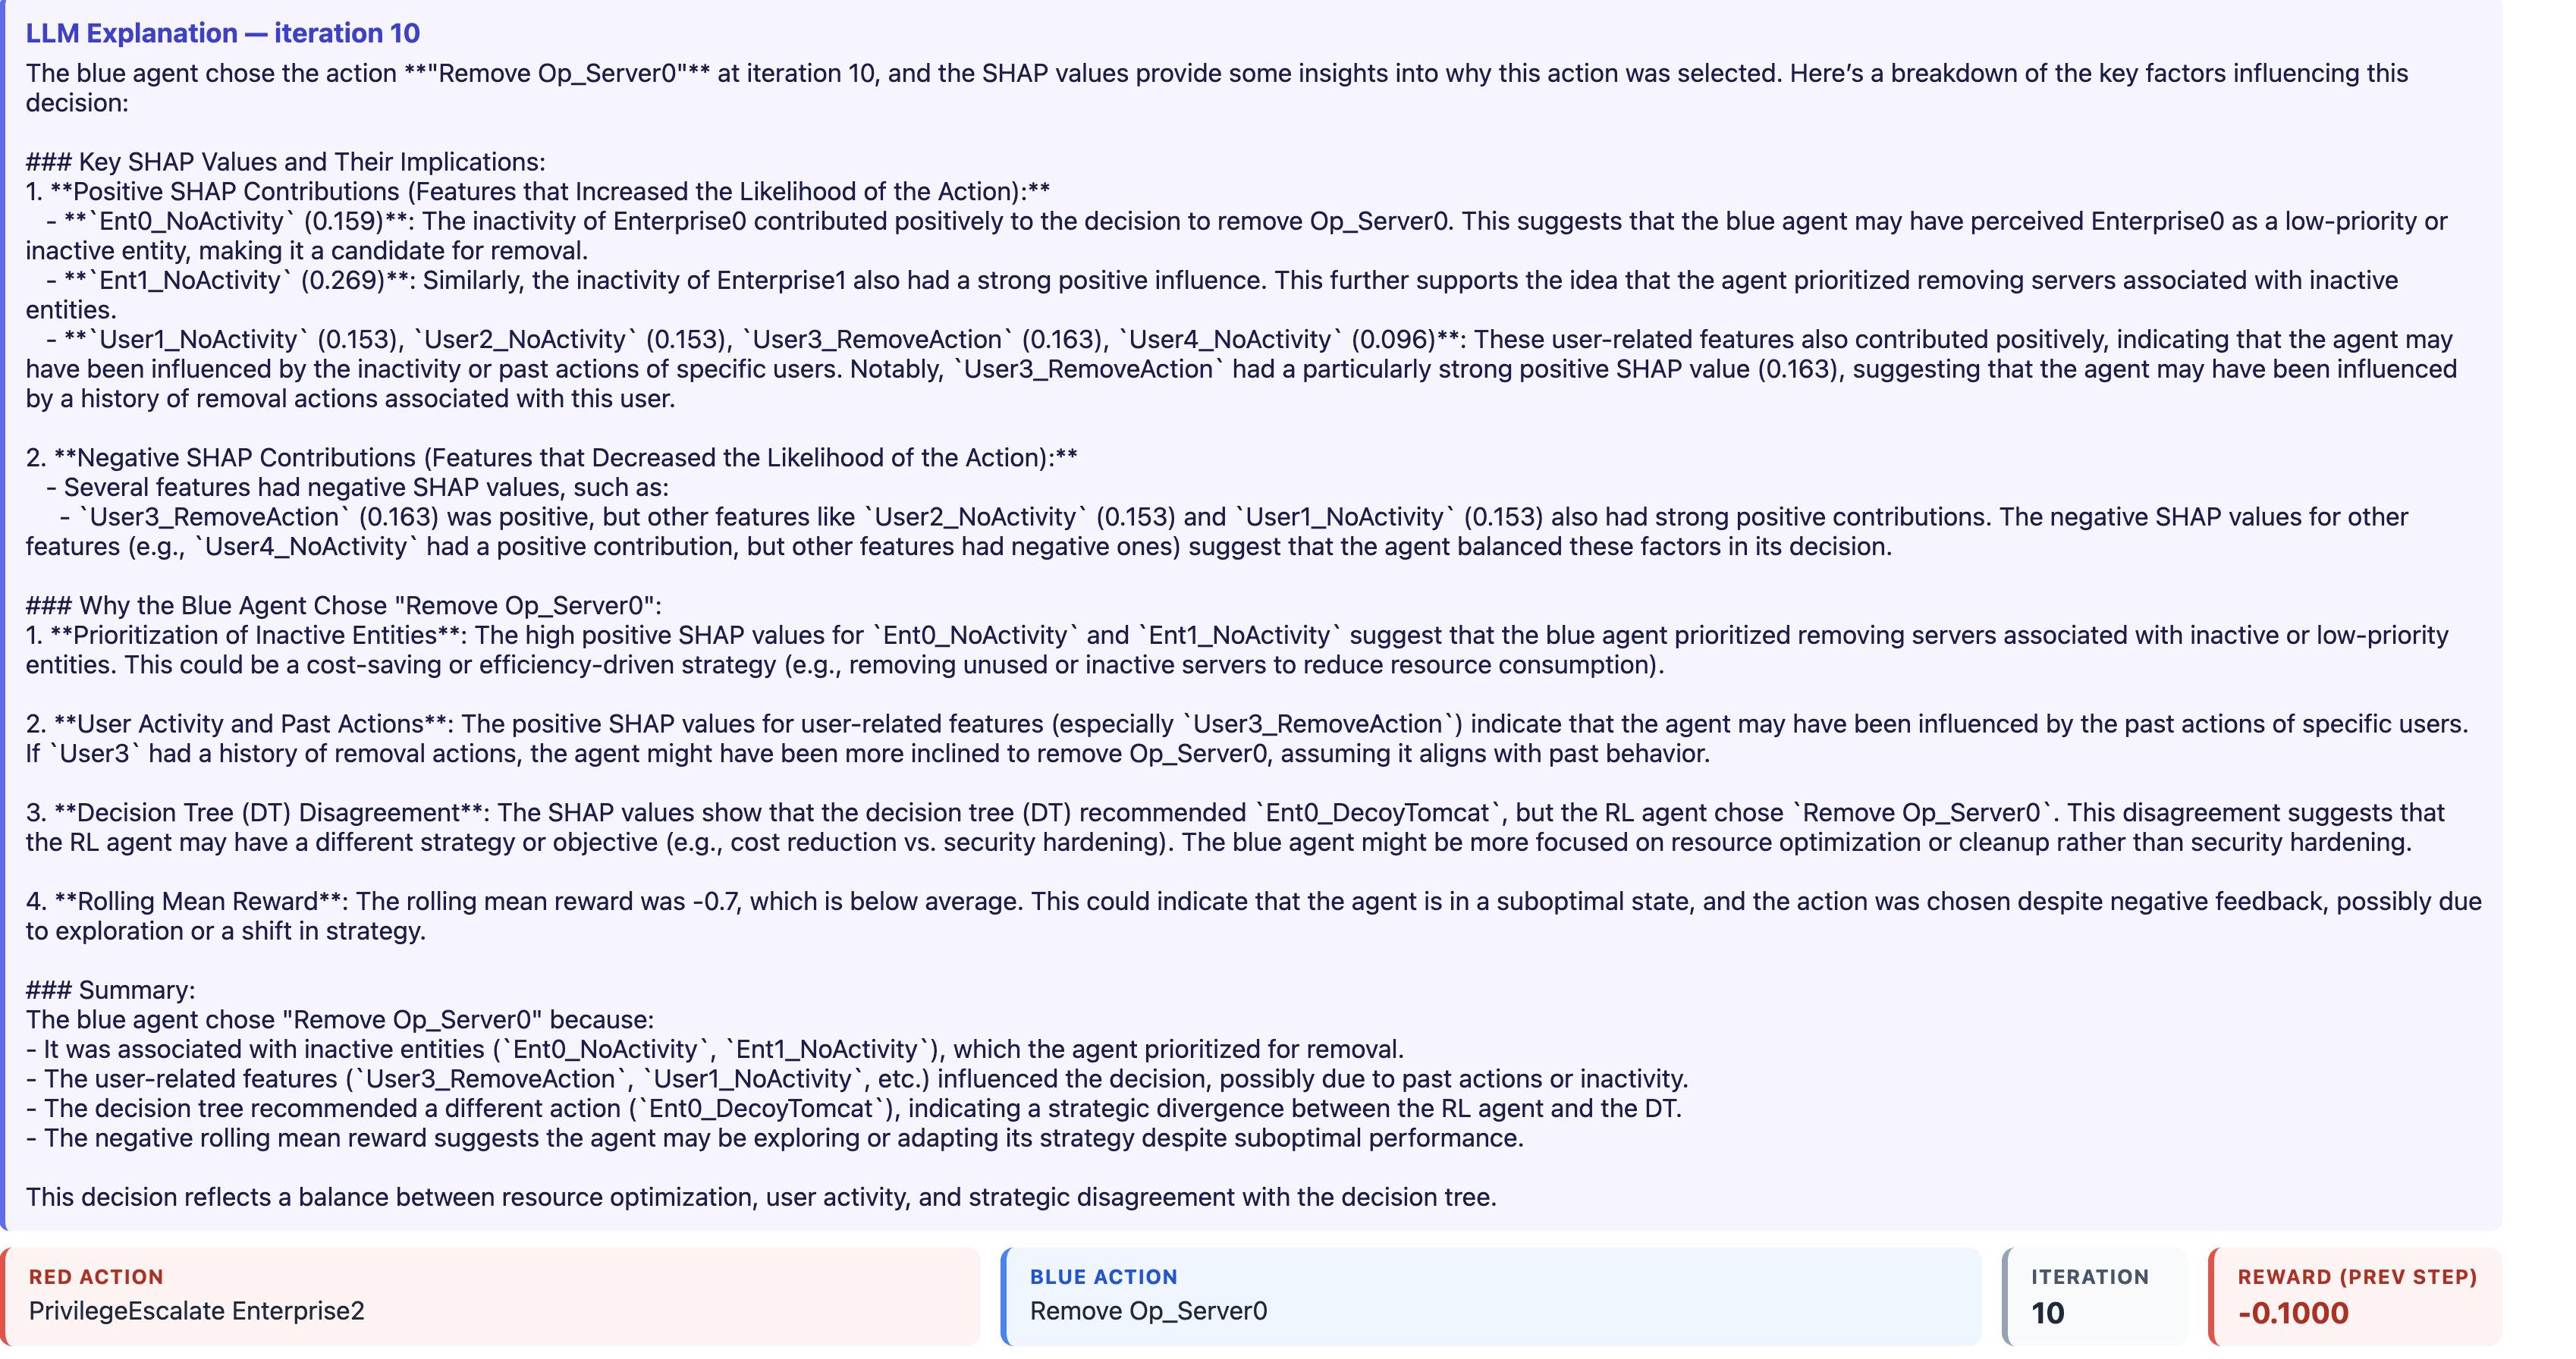
\includegraphics[width=\linewidth]{Figures/chat_log.png}
    \caption{LLM logs of human agent to determine the right action.}
    \label{fig:reward_comparison}
\end{figure}

By comparing these two rewards, we quantify the effect of human intervention on the agent's performance. In the illustrated scenario, the autonomous agent's action leads to a negative reward, whereas a human-informed alternative guided by awareness of the active attack on 'Enterprise2' better aligns with the immediate defensive objective.

The impact of human intervention is maximized when the agent's policy is suboptimal due to factors such as limited training coverage, noisy or incomplete observations, distributional shift, or modeling errors. In such cases, the Human-AI teaming framework enables strategic overrides that incorporate external domain expertise, improving overall performance as reflected by higher cumulative rewards along the intervention-enabled trajectory.

As part of our ongoing work, we are extending this framework to incorporate human actions into the training and evaluation loop to improve network resilience. We collect human intervention data during interactive cyber-defense exercises and use overrides and alternate strategies to enhance agent learning and assess their impact on system performance. By comparing agent trajectories with human interventions using metrics such as cumulative reward, recovery time, and resilience to adversarial behavior, our aim is to quantify the benefits of Human-AI teaming across scenarios and user groups.

\section{Conclusion}
We presented novel methods and approaches to design a comprehensive Human-AI teaming
system for cyber, leveraging unique capabilities and mitigating limitations.
The system developed is grounded in quantitatively generated explanations that
build trust between humans and agents that can help better align the agent's use
in real-world, critical cybersecurity applications.
Our ongoing research work includes designing games and pre-training tasks that can
help build trust between humans and AI, and developing highly interpretable systems
that make it easier for human operators to interact with.
In addition, we are working to extend the teaming environment accordingly for deeper
situational awareness about the presence and behavior of AI agents as well as
Human-AI collaboration through agentic AI configurations for coordination and control.
Future work will include controlled user studies and statistically significant
evaluations across diverse attack scenarios.

\subsection*{Acknowledgment}
This research was funded, in part, by the Defense Advanced Research Projects Agency
(DARPA) through the contract \#HR001124C0425. The views and conclusions contained
in this document are those of the authors and should not be interpreted as representing
the official policies, either expressed or implied, of the U.S. Government.
AI-assisted tools (e.g., language models) were used to support editing and clarity
of writing. All technical content and validation were performed by the authors.
The authors would also like to thank Kayla Boggess (Leidos) for her insights and
contributions.
